% ----------------------------------------------------------
% APÊNDICE A - Algorithms
% ----------------------------------------------------------
\begin{apendicesenv}
\chapter{Algorithms}
\label{app:algorithms}
\subsection*{BinomialDistribution\_PROB and Distribution\_PROB}
%\enlargethispage{40mm}
The BinomialDistribution\_PROB algorithm generates the probability of distribution of an interval and uses the general binomial probability formula below. This algorithm has the same result as the Distribution\_PROB algorithm, but the BinomialDistribution\_PROB execution is much faster and has higher capacity because it uses large numbers like BigInteger and BigDecimal. Both algorithms were done in C\# with LINQPad 5 \footnotemark. The Figure \ref{fig:BinomialDistribution_PROB_and_Distribution_PROB} shows the results of the algorithms for the range 0 to 10, analogous to flipping 10 coins on the ground, adding up the values of the heads and tails, with the tails having the value one and the heads having the value two. The Distribution\_PROB algorithm sums each of the 1024 possibilities [1,1,1,1,1,1,1,1,1,1,1,1 - 1,1,1,1,1,1,1,1,1,1,1, 2 - ....] and groups these values together. In the Distribution\_PROB algorithm, this set of possibilities is a Cartesian product of the possible combinations, which makes this algorithm slow, but it is important to validate and facilitate understanding of the general binomial probability formula used in the BinomialDistribution\_PROB algorithm \cite{mathisfun_binomial_distribution}. In the Figure \ref{fig:BinomialDistribution_PROB_and_Distribution_PROB}, the table within Distribution\_PROB shows this grouping and the total number of possibilities, 1024. Dividing each grouped value by the total gives the probabilistic result achieved by the formula used in BinomialDistribution\_PROB. For example, the probability that the sum of the 10 coins flipped is 12 is equal to 45/1024, or 0.0439453125 or 4.39\%.
\footnotetext{LINQPad 5 is on \url{www.linqpad.net} and can be used in its free version (Standard edition) without expiration.}
%\enlargethispage{-50mm}
	\begin{align*}
	f(k;n,p) &= \binom{n}{k} p^k(1 - p)^{n-k}
	\end{align*}
	\begin{figure}[H]
	\caption{Results of the BinomialDistribution\_PROB and Distribution\_PROB algorithms}
	\label{fig:BinomialDistribution_PROB_and_Distribution_PROB}
	\centering
	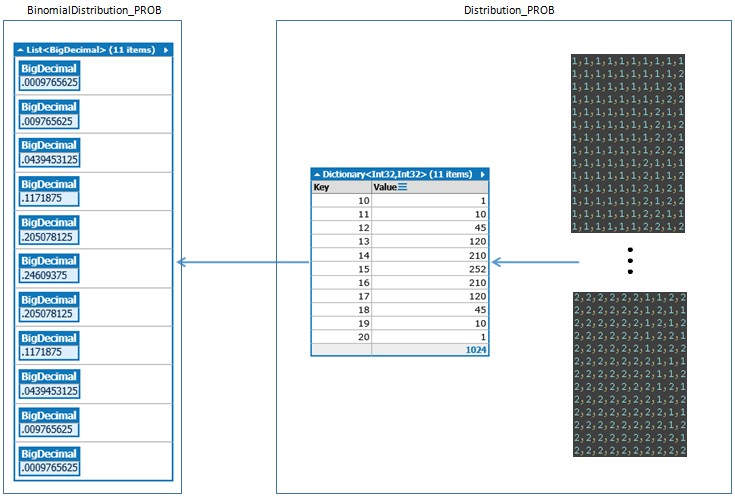
\includegraphics[scale=.77]{sections/images/BinomialDistribution_PROB_and_Distribution_PROB.jpg}
	\floatfoot{The Distribution\_PROB algorithm intends to clarify the probabilistic essence of the central limit theorem.} %\footnotemark.
	\end{figure}

The Distribution\_PROB algorithm can also be used for the roll of 5 6-sided dice or 6 5-sided dice, for example. As can be seen in the Figure below, the probability distribution on the dice roll is similar to the binomial distribution (coins).
	\begin{figure}[H]
	\centering
		\begin{subfigure}[H]{0.47\linewidth}
		\centering
		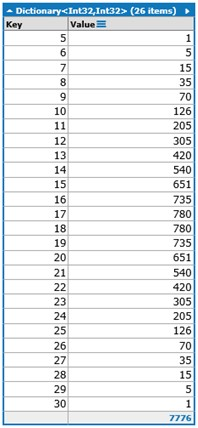
\includegraphics[width=.6\linewidth]{sections/images/Distribution_PROB_5_6.jpg}
		\caption{5 6-sided dice}
		\label{fig:Distribution_PROB_5_6}
		\end{subfigure}
	\hfill
		\begin{subfigure}[H]{0.47\linewidth}
		\centering
		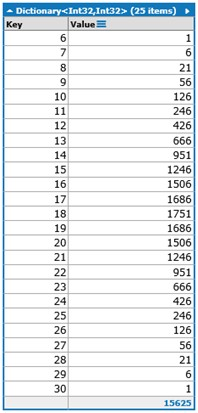
\includegraphics[width=.62\linewidth]{sections/images/Distribution_PROB_6_5.jpg}
		\caption{6 5-sided dice}
		\label{fig:Distribution_PROB_6_5}
		\end{subfigure}%
	\caption{Results of the Distribution\_PROB algorithm}
	\floatfoot{The probability distribution on the dice roll is consonant to the binomial distribution.} %\protect\footnotemark
	\end{figure}

\subsubsection*{BinomialDistribution\_PROB [Code]}
To execute the code snippet requires the implementation of BigDecimal, an example of that implementation can be seen, obeying proprietary software license rights, at \cite{github_bigdecimal}. This study does not distribute nor is it responsible for the portion of the code related to the BigDecimal implementation, these responsibilities being the responsibility of the executor of this software.

\bigbreak
\begin{lstlisting}
//https://www.mathsisfun.com/data/quincunx-explained.html
void Main()
{
    BinomailDistribuition.Possibilities = 10;
    var results = new List<BigDecimal>();
    results.Load();
    results.Print(true); //send false to print Table 1.
}

public static class BinomailDistribuition
{
    public static int Possibilities = 0;
    static int middleLeft = 0;
    static int middleRight = 0;
    static int resultCount = 0;
    
    public static void Load(this List<BigDecimal> results)
    {
        for (int i = 0; i <= Possibilities; i++)
        {
            var fatorLeft = Fatorial(Possibilities);
            var fatorRight = BigInteger.Multiply(Fatorial(i), Fatorial(Possibilities - i));
            BigInteger fat = BigInteger.Divide(fatorLeft, fatorRight);
            var powLeft = new BigDecimal(1, 0, 1000000000);
            var powRight = new BigDecimal(1, 0, 1000000000);
            if (i != 0)
                powLeft = BigDecimal.Pow(new BigDecimal(5, 1, 1000000000), i);
            if (i != Possibilities)
                powRight = BigDecimal.Pow(new BigDecimal(5, 1, 1000000000), (Possibilities - i));
            var prob = new BigDecimal(fat) * powLeft * powRight;
            results.Add(prob);
        }
    }
    
    public static BigInteger Fatorial(int value)
    {
        BigInteger fatorial = 1;
        for (int n = 1; n <= value; n++)
        {
            fatorial *= n;
        }
        return fatorial;
    }
    
    public static void Print(this List<BigDecimal> results, bool printTableProbability)
    {
        if (!printTableProbability)
        {
            var sum = results.Sum();
            var middle = (middleRight - middleLeft) / 2;
            var middlePercent = ((middleRight - middleLeft) * 14) / 100;
            var list = results.Where((x, i) => i >= middleLeft && i <= middleRight).ToList();
            var listPareto = list.Where((x, i) => i >= (middle - middlePercent) && i <= (middle + middlePercent)).ToList();
            var percentOfSum = (middleRight - middleLeft) * 100 / resultCount;
            var sumPercent = sum * new BigDecimal(100, 0, 1000000000);
            var paretoResult = new BigDecimal(0, 0, 1000000000);
            listPareto.ForEach(x => { paretoResult = paretoResult + x; });

            sumPercent.Dump("sum");
            middleLeft.Dump("middleLeft");
            middleRight.Dump("middleRight");
            (middleRight - middleLeft).Dump("itens of sum");
            percentOfSum.Dump("percent of sum");
            resultCount.Dump("total");
            paretoResult.Dump("20/80");
        }
        else
        {
            results.Dump(); //Valid Binomial distribution    
        }
    }
    
    public static BigDecimal Sum(this List<BigDecimal> results)
    {
        resultCount = results.Count;
        middleLeft = resultCount / 2;
        middleRight = middleLeft * 2 < resultCount ? middleLeft + 1 : middleLeft;

        var sum = middleLeft != middleRight ? results[middleLeft] + results[middleRight] : results[middleRight];
        while ((sum * new BigDecimal(100, 0, 1000000000)) < new BigDecimal(9999, 2, 1000000000))
        {
            middleLeft--;
            middleRight++;
            if (middleLeft >= 0)
                sum = sum + results[middleLeft];
            if (middleRight <= Possibilities)
                sum = sum + results[middleRight];
        }
        return sum;
    }
}

//Exemple of BigDecimal class - https://github.com/dparker1/BigDecimal/blob/
//3e0a4f1ba4c72c0b28d6571fcc6259558be104bd/BigDecimal/BigDecimal.cs
\end{lstlisting}

\bigbreak
\bigbreak
\subsubsection*{Distribution\_PROB [Code]}
\begin{lstlisting}
//https://exercicios.brasilescola.uol.com.br/exercicios-matematica/
//exercicios-sobre-probabilidade-condicional.htm#questao-1
void Main()
{
    var dice = 2; //Binomial distribution, dice = 2;
    var events = 10;
    var sampling = Math.Pow(dice, events);
    var cartesianProduct = dice.ToArrays(events).CartesianProduct();
    cartesianProduct.PrintGroup(events, dice);
}

public static class CartesianProductContainer
{
    public static IEnumerable<IEnumerable<int>> CartesianProduct(this IEnumerable<IEnumerable<int>> sequences)
    {
        IEnumerable<IEnumerable<int>> emptyProduct = new[] { Enumerable.Empty<int>() };
        var result = sequences.Aggregate(
            emptyProduct,
            (accumulator, sequence) =>
                from accseq in accumulator
                from item in sequence
                select new[] { accseq.Concat(new[] { item }).Sum() });

        return result;
    }

    public static IEnumerable<List<int>> ToArrays(this int dice, int events)
    {
        var result = new List<List<int>>();
        for (int j = 1; j <= events; j++)
        {
            var array = new List<int>();
            for (int i = 1; i <= dice; i++)
                array.Add(i);
            
            result.Add(array);
        }

        return result;
    }
    
    public static void PrintGroup(this IEnumerable<IEnumerable<int>> list, int events, int dice)
    {
        var listCountDict = Enumerable.Range(1, dice * events).ToDictionary(x => x);
        Group(listCountDict, list);
        listCountDict.Dump("Values");
    }

    public static void Group(Dictionary<int, int> dict, IEnumerable<IEnumerable<int>> list)
    {
        foreach (var key in dict.Keys.ToList())
            dict[key] = 0;

        foreach (var item in list)
            dict[item.First()]++;

        var zeroKey = 0;
        foreach (var item in dict)
            if (item.Value == 0) 
                zeroKey = item.Key;
            else continue;

        for (int i = 1; i <= zeroKey; i++)
            dict.Remove(i);
    }
}

\end{lstlisting}


\bigbreak \bigbreak
\subsection*{Logic\_WavePattern}
The Logic\_WavePattern algorithm results in the display of a histogram that assumes the wave pattern when placed side by side each of the bars on the left and right side of the median. This histogram is generated from randomizing the values according to Figure \ref{fig:consciousness_logical_moments} and Figure \ref{fig:consciousness}, following the central limit theorem.
	\begin{figure}[H]
	\caption{Histogram in the wave pattern of the Logic\_WavePattern algorithm}
	\label{fig:logic_wavepattern_15000}
	\centering
	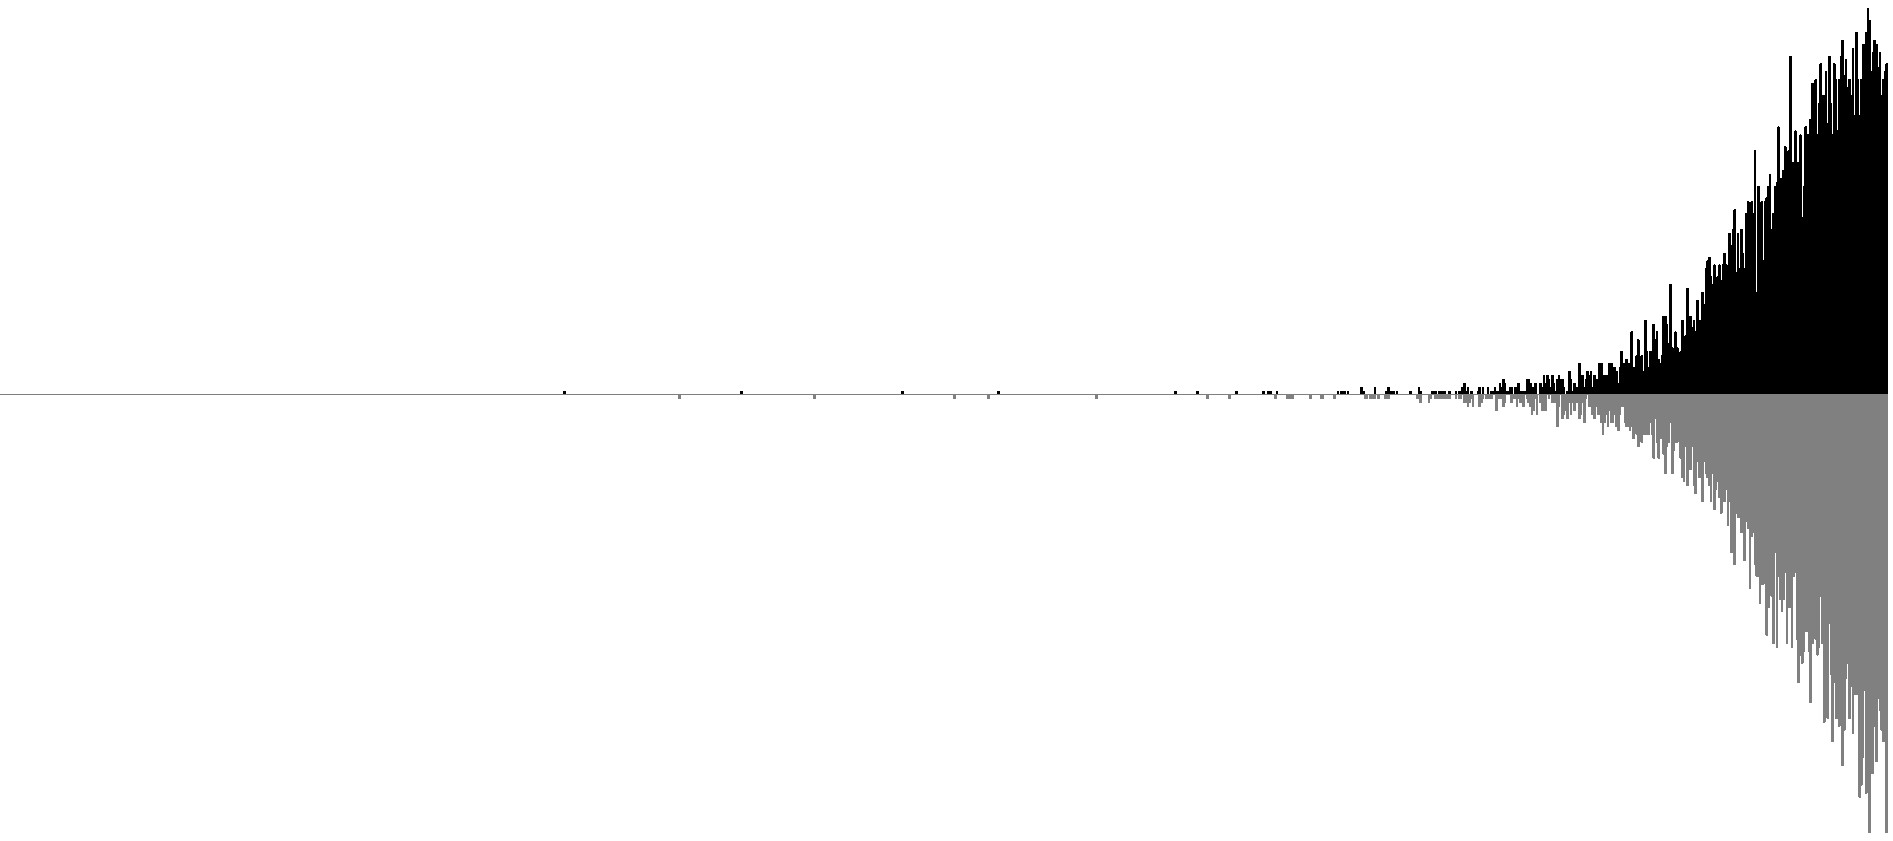
\includegraphics[scale=.25]{sections/images/logic_wavepattern_15000.jpg}
	\floatfoot{Randomly generated result displayed by the Logic\_WavePattern algorithm.} %\footnotemark.
	\end{figure}

Another result of the Logic\_WavePattern algorithm is obtained from the LINQPad 5 console, which outputs a file in ".csv" format that can be imported into Plotly's Chart Studio \url{https://chart-studio. plot.ly/create} for generating a 3D scatter plot. The most important part of the graph are the points that represent the most easily visible part and that are most likely at the top of each histogram bar in the previous Figure. Lines are used to facilitate the visualization of spirals that are already starting to form even with very low volumes of data and without the entanglement of intervals (ordering).
	\begin{figure}[H]
	\caption{3D scatter plot of the Logic\_WavePattern algorithm}
	\label{fig:plotly_3DScatter}
	\centering
	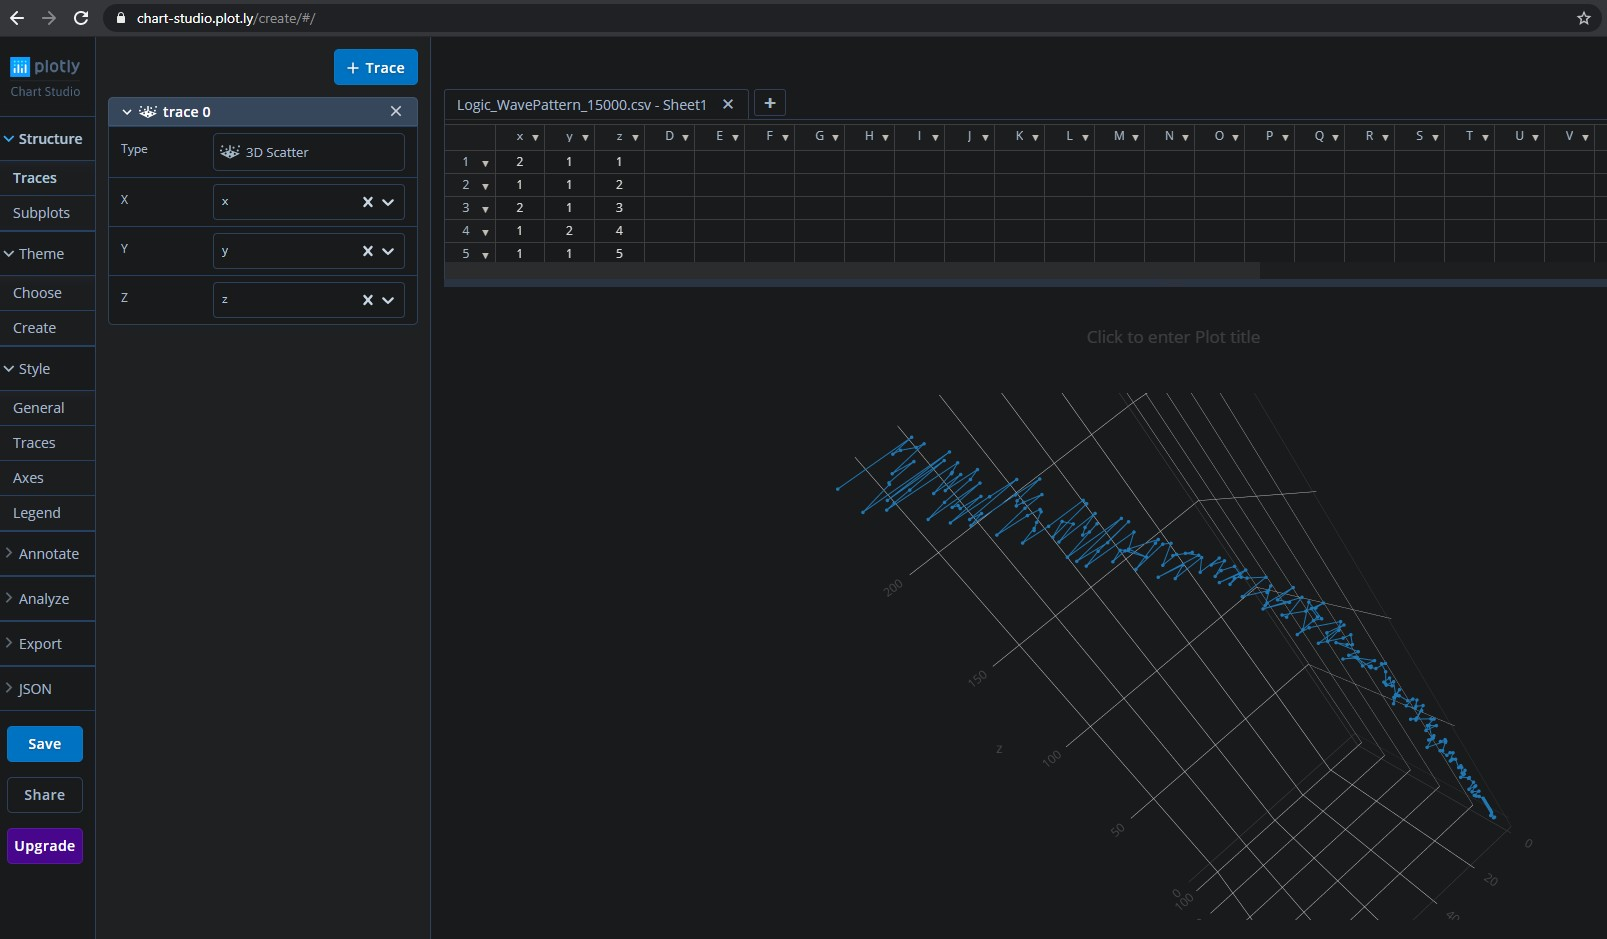
\includegraphics[scale=.33]{sections/images/plotly_3DScatter.jpg}
	\floatfoot{The example can be accessed at: \url{https://chart-studio.plot.ly/create/?fid=ren.stuchi:5&fid=ren.stuchi:4}.} %\footnotemark.
	\end{figure}

\subsubsection*{Logic\_WavePattern [Code]}
\begin{lstlisting}
//http://csharphelper.com/blog/2015/09/draw-a-simple-histogram-in-c/
//https://github.com/naudio/NAudio.WaveFormRenderer
[STAThread]
void Main()
{
  Application.EnableVisualStyles();
  Application.Run(new MainForm());
}

public partial class MainForm : Form
{
  public MainForm()
  {
    InitializeComponent();
  }
  //###########################################################################
  private const int LENGHT = 30000;
  private const int GROUP = 2;
  //###########################################################################
  private double m_dZoomscale = 1.0;
  public static double s_dScrollValue = .25;
  private Point MouseDownLocation;
  private Matrix transform = null;
  private NumbsOfCentralLimitTheorem.HistogramResult histogramResult = null;
  private bool printed = false;

  private void MainForm_Load(object sender, EventArgs e)
  {
    histogramResult = GetHistogramOfCentralLimitTheorem(LENGHT, GROUP);

    RectangleF data_bounds = new RectangleF(0, 0, histogramResult.Size, histogramResult.MaxValue * 2);
    PointF[] points =
    {
        new PointF(0, pictHistogram.ClientSize.Height),
        new PointF(pictHistogram.ClientSize.Width, pictHistogram.ClientSize.Height),
        new PointF(0, 0)
      };
    transform = new Matrix(data_bounds, points);
  }

  private void pictHistogram_Paint(object sender, PaintEventArgs e)
  {
    DrawHistogram(e.Graphics, pictHistogram.BackColor, histogramResult,
      pictHistogram.ClientSize.Width, pictHistogram.ClientSize.Height);
  }

  private void pictHistogram_Resize(object sender, EventArgs e)
  {
    pictHistogram.Refresh();
  }

  private void DrawHistogram(Graphics gr, Color back_color,
    NumbsOfCentralLimitTheorem.HistogramResult histogramResult, int width, int height)
  {
    PrintResult();
    gr.Clear(back_color);
    gr.Transform = transform;
    gr.ScaleTransform((float)m_dZoomscale, (float)m_dZoomscale);
    FillRectangle(gr, Color.Black, histogramResult.Up, histogramResult.MaxValue, false);
    FillRectangle(gr, Color.Gray, histogramResult.Down, histogramResult.MaxValue, true);
  }

  private void PrintResult()
  {
    if (!printed)
    {
      printed = true;
      var listTuple = new List<(float x, float y, float z)>();
      float previousValueOfZ = 0;
      for (int i = 0; i < histogramResult.Up.Count(); i++)
      {
        if (histogramResult.Up[i] != 0.0001f && histogramResult.Down[i] != 0.0001f)
        {
          if (histogramResult.Up[i] % 1 == 0)
            previousValueOfZ = (int)(previousValueOfZ + 1f);
          else
            previousValueOfZ += 0.1f;
          var tuple = (x: histogramResult.Up[i], y: histogramResult.Down[i], z: previousValueOfZ);
          listTuple.Add(tuple);
        }
      }
      Console.WriteLine("x,y,z");
      foreach (var tuple in listTuple)
        Console.WriteLine(tuple.x.ToString() + "," + tuple.y.ToString() + "," + tuple.z.ToString());
    }
  }

  protected void FillRectangle(Graphics gr, Color color, float[] arrayValues, float maxValue, bool down)
  {
    using (Pen thin_pen = new Pen(color, 0))
    {
      for (int i = 0; i < histogramResult.Down.Length; i++)
      {
        RectangleF rect;
        if (!down)
          rect = new RectangleF(i, maxValue, 1, arrayValues[i]);
        else
          rect = new RectangleF(i, maxValue - arrayValues[i], 1, arrayValues[i]);
        using (Brush the_brush = new SolidBrush(color))
        {
          gr.FillRectangle(the_brush, rect);
          gr.DrawRectangle(thin_pen, rect.X, rect.Y, rect.Width, rect.Height);
        }
      }
    }
  }

  protected void pictHistogram_OnMouseWheel(object sender, MouseEventArgs mea)
  {
    pictHistogram.Focus();
    if (pictHistogram.Focused == true && mea.Delta != 0)
      ZoomScroll(mea.Location, mea.Delta > 0);
  }

  private void ZoomScroll(Point location, bool zoomIn)
  {
    transform.Translate(-location.X, -location.Y);
    if (zoomIn)
      m_dZoomscale = m_dZoomscale + s_dScrollValue;
    else
      m_dZoomscale = m_dZoomscale - s_dScrollValue;
    transform.Translate(location.X, location.Y);
    pictHistogram.Invalidate();
  }

  private void pictHistogram_MouseDown(object sender, MouseEventArgs e)
  {
    if (e.Button == System.Windows.Forms.MouseButtons.Left)
      MouseDownLocation = e.Location;
  }

  private void pictHistogram_MouseMove(object sender, MouseEventArgs e)
  {
    if (e.Button == System.Windows.Forms.MouseButtons.Left)
    {
      transform.Translate((e.Location.X - MouseDownLocation.X)
        / 40, (e.Location.Y - MouseDownLocation.Y) / 40, MatrixOrder.Append);
      this.Refresh();
    }
  }

  private NumbsOfCentralLimitTheorem.HistogramResult GetHistogramOfCentralLimitTheorem(int length, int group)
  {
    var numbsOfCentralLimitTheorem = new NumbsOfCentralLimitTheorem();
    numbsOfCentralLimitTheorem.RandomResult(length);
    return numbsOfCentralLimitTheorem.GenerateHistogram(group);
  }
}

partial class MainForm
{
  private System.ComponentModel.IContainer components = null;

  protected override void Dispose(bool disposing)
  {
    if (disposing && (components != null))
      components.Dispose();
    base.Dispose(disposing);
  }

  private void InitializeComponent()
  {
    this.pictHistogram = new System.Windows.Forms.PictureBox();
    ((System.ComponentModel.ISupportInitialize)(this.pictHistogram)).BeginInit();
    this.SuspendLayout();
    this.pictHistogram.Anchor = ((System.Windows.Forms.AnchorStyles)((((System.Windows.Forms.AnchorStyles.Top
          | System.Windows.Forms.AnchorStyles.Bottom)
          | System.Windows.Forms.AnchorStyles.Left)
          | System.Windows.Forms.AnchorStyles.Right)));
    this.pictHistogram.BackColor = System.Drawing.Color.White;
    this.pictHistogram.Cursor = System.Windows.Forms.Cursors.Cross;
    this.pictHistogram.Location = new System.Drawing.Point(8, 6);
    this.pictHistogram.Name = "pictHistogram";
    this.pictHistogram.Size = new System.Drawing.Size(550, 250);
    this.pictHistogram.TabIndex = 1;
    this.pictHistogram.TabStop = false;
    this.pictHistogram.Resize += new System.EventHandler(this.pictHistogram_Resize);
    this.pictHistogram.Paint += new System.Windows.Forms.PaintEventHandler(this.pictHistogram_Paint);
    this.pictHistogram.MouseWheel += new System.Windows.Forms.MouseEventHandler(this.pictHistogram_OnMouseWheel);
    this.pictHistogram.MouseDown += new System.Windows.Forms.MouseEventHandler(this.pictHistogram_MouseDown);
    this.pictHistogram.MouseMove += new System.Windows.Forms.MouseEventHandler(this.pictHistogram_MouseMove);
    this.AutoScaleDimensions = new System.Drawing.SizeF(6F, 13F);
    this.AutoScaleMode = System.Windows.Forms.AutoScaleMode.Font;
    this.ClientSize = new System.Drawing.Size(563, 262);
    this.Controls.Add(this.pictHistogram);
    this.Name = "MainForm";
    this.Text = "Logic_WavePattern";
    this.Load += new System.EventHandler(this.MainForm_Load);
    ((System.ComponentModel.ISupportInitialize)(this.pictHistogram)).EndInit();
    this.ResumeLayout(false);
  }

  internal System.Windows.Forms.PictureBox pictHistogram;
}

public class NumbsOfCentralLimitTheorem
{
  public float[] ResultList { get; set; }
  public int ResultLength { get; set; }
  public float[] LastList { get; set; }
  public float[] CurrentList { get; set; }
  public int SizeLastList { get; set; }
  public Dictionary<int, float> Histogram { get; set; }

  public NumbsOfCentralLimitTheorem()
  {
    SizeLastList = 2;
    StartLastList();
    StartCurrentList();
  }

  public float[] RandomResult(int length)
  {
    ResultLength = length;
    ResultList = new float[length];
    Random rnd = new Random();
    for (int x = 0; x < length; x++)
    {
      float lineSum = 0;
      for (int i = 1; i < SizeLastList; i++)
      {
        var lastValueLeft = LastList[i - 1];
        var lastValueRight = LastList[i];
        var rndValue = (float)rnd.NextDouble(lastValueLeft, lastValueRight);
        lineSum = lineSum + (rndValue - lastValueLeft);
        CurrentList[i] = rndValue;
      }
      if (lineSum != 0)
        ResultList[x] = lineSum;
      SizeLastList++;
      LastList = CurrentList;
      StartCurrentList();
    }
    return ResultList;
  }

  public HistogramResult GenerateHistogram(int group)
  {
    Histogram = new Dictionary<int, float>();
    var minValue = ResultList.Min();
    var maxValue = ResultList.Max();
    var rangeValue = maxValue - minValue;
    var amountOfGroups = ResultLength / group;
    var intervalValue = rangeValue / amountOfGroups;
    foreach (var value in ResultList)
    {
      int key = (int)(value / intervalValue);
      if (!Histogram.ContainsKey(key))
        Histogram[key] = 0;
      Histogram[key]++;
    }
    var histogramResult = HistogramResult.Get(Histogram);
    return histogramResult;
  }

  private void StartCurrentList()
  {
    var sizeCurrentList = SizeLastList + 1;
    CurrentList = new float[sizeCurrentList];
    CurrentList[0] = 0;
    CurrentList[sizeCurrentList - 1] = float.MaxValue / 2; 
  }

  private void StartLastList()
  {
    LastList = new float[SizeLastList];
    LastList[0] = 0;
    LastList[SizeLastList - 1] = float.MaxValue / 2; 
  }

  public class HistogramResult
  {
    public int Size { get; set; }
    public float MaxValue { get; set; }
    public float[] Up { get; set; }
    public float[] Down { get; set; }

    public static HistogramResult Get(Dictionary<int, float> histogram)
    {
      var histogramOrdered = histogram.OrderBy(k => k.Key);
      var result = new HistogramResult();
      var lengthOdd = histogram.Count % 2 > 0;
      var middle = histogram.Count / 2;
      var middleValue = histogramOrdered.ElementAt(middle).Key;
      result.Size = middleValue;
      result.MaxValue = histogram.OrderBy(k => k.Value).Last().Value;
      result.Up = ArrangeArray(new float[middleValue]);
      result.Down = ArrangeArray(new float[middleValue]);
      for (int i = 0; i < middle; i++)
      {
        var keyValue = histogramOrdered.ElementAt(i);
        result.Up[keyValue.Key] = keyValue.Value;
      }
      for (int i = lengthOdd ? middle + 2 : middle + 1; i < histogram.Count; i++)
      {
        var totalValue = middleValue * 2;
        var keyValue = histogramOrdered.ElementAt(i);
        result.Down[totalValue - keyValue.Key] = keyValue.Value;
      }
      return result;
    }

    private static float[] ArrangeArray(float[] array)
    {
      for (int i = 0; i < array.Length; i++)
        array[i] = 0.0001F;
      return array;
    }
  }
}

public static class rndExtension
{
  public static double NextDouble(this Random rng, double minimum, double maximum)
  {
    return rng.NextDouble() * (maximum - minimum) + minimum;
  }
}
\end{lstlisting}

\end{apendicesenv}